\subsection{工厂方法模式(Factory Method)}

\subsubsection{工厂方法模式简介}

工厂方法模式是一种创建型设计模式,它提供了一种创建对象的最佳方式。在工厂方法模式中,通过定义工厂类来负责创建具体的对象,通过传递不同的参数来创建不同的对象。工厂方法模式的优点是可以将对象的创建和使用分离,通过使用不同的工厂类来创建不同的对象,可以提高系统的灵活性和可扩展性。

要实现工厂方法模式,需要定义一个抽象工厂类来声明创建对象的接口,并定义一个具体工厂类来实现抽象工厂类中声明的创建对象的方法。通常,抽象工厂类和具体工厂类都需要实现一个接口或抽象类,该接口或抽象类定义了具体的对象所具有的功能。

工厂方法模式有一些优点:

可以将对象的创建和使用分离,使系统更加灵活和可扩展。

在工厂方法模式中,客户端可以通过传递不同的参数来创建不同的对象,并且不需要关心对象的创建细节。

工厂方法模式提供了一种更好的扩展方式。

好的,那么工厂方法模式还有一些缺点:

在工厂方法模式中,如果需要增加新的产品,则需要修改抽象工厂类和具体工厂类,这违背了开闭原则。

在工厂方法模式中,增加新的产品时需要对抽象工厂类进行修改,这会导致抽象工厂类变得臃肿,不利于维护。

通常,工厂方法模式适用于以下场景:

创建对象的任务由多个具体子类中的某一个来完成,由客户端决定实例化哪一个具体子类。

需要将对象的创建和对象的使用分离。

在实际开发中,应根据实际情况来判断是否使用工厂方法模式。如果需要将对象的创建和使用分离,并且希望通过传递不同的参数来创建不同的对象,那么可以考虑使用工厂方法模式来实现这个功能。

\subsubsection{工厂方法模式在项目中的应用}

\begin{figure}[htb]
  \centering
  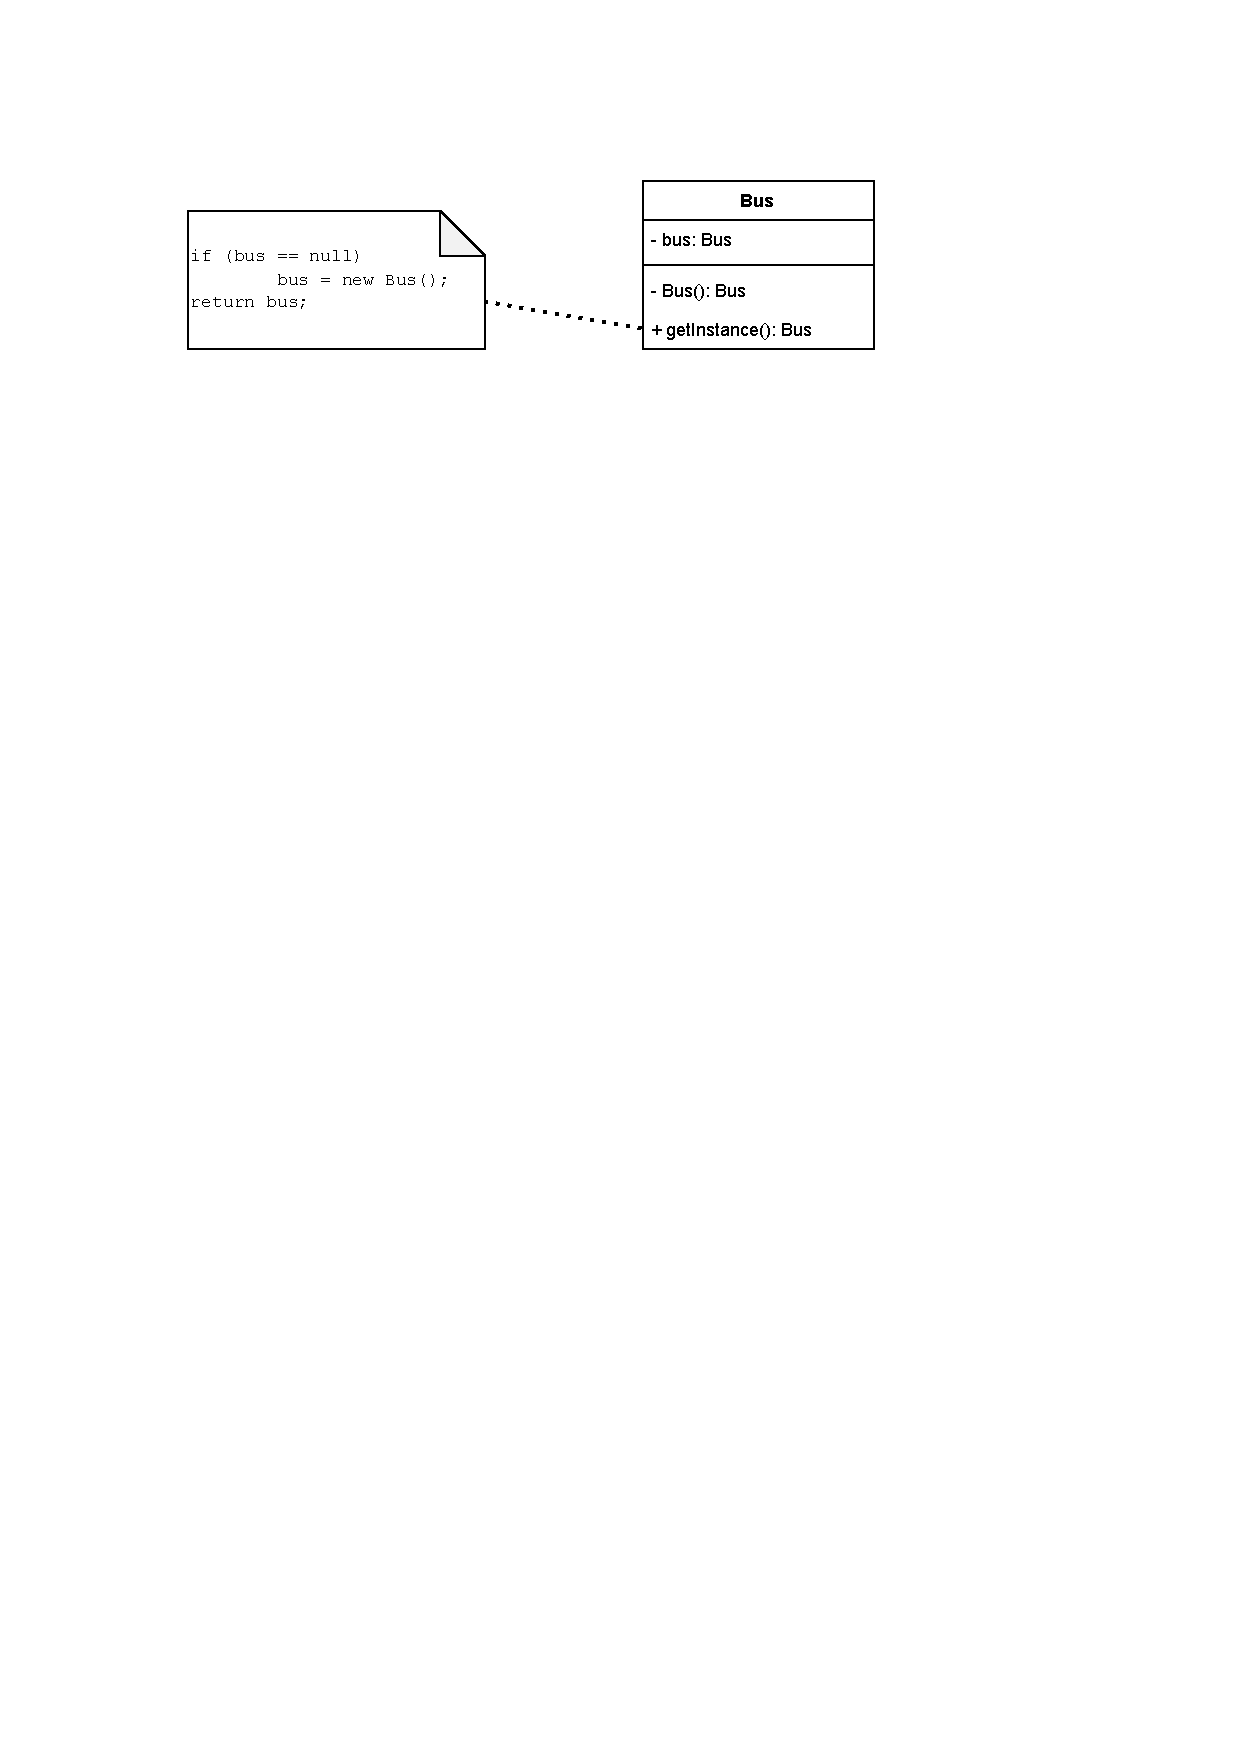
\includegraphics[width=0.9\textwidth]{figures/单例.pdf}
  \caption{工厂方法模式在 Slow6502 中的类图}
\end{figure}

我们的Memory类使用了工厂模式,两个属于Memory的类(RAM,ROM)可以通过MemoryFactory创建。使用工厂模式可以使得在创建 Memory 类的实例时,将具体的内存创建过程隔离出来。这样,如果你希望更改内存创建的方式,比如使用不同的类型的内存或者使用不同的方法来创建内存,只需要修改工厂类的代码,而不需要修改 Memory 类的代码。这样可以让你更方便地扩展和修改项目,并且降低了代码的耦合度。

